\textbf{Код задачи №26695}

\lstinputlisting{paragrafs/Zadachi/11}

Одной из особенностей этого шаблона является, использующаяся в нём библиотека \texttt{setMinimaxFunctionTask}, которая берёт на себя большую часть работы по подбору значейний, а также отображению задачи на экране. Но всё же трудности могут возникнуть при подборе значений для  \texttt{primaryStep:} и \texttt{secondaryStep:}, отвещающих за первичный и вторичный перебор значений максимума или минимума соответственно. Сначала поиск проходит первичным шагом, затем в окрестности предполагаемого ответа, происходит поиск вторичным шагом. Чем меньше задать шаги поиска, тем больше будет нагрузка и дольше программа будет подбирать значение, а если сделать наоборот, и задать шаги большего размера, то увеличится скорость поиска, но пострадает точность решения.


\textbf{Задания сгенерированные по шаблону задачи №26695.}
	\begin{figure}[h]
		\centering
		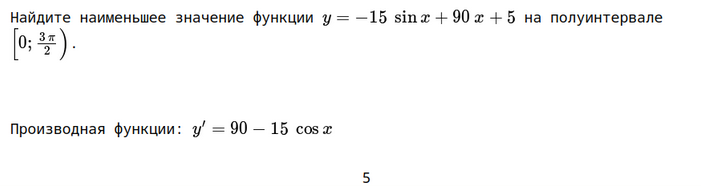
\includegraphics[width=1\linewidth]{VM/p1.png}
		
\includegraphics[width=1.01\linewidth]{VM/aaa.jpeg}
	\end{figure}

	
